% Options for packages loaded elsewhere
\PassOptionsToPackage{unicode}{hyperref}
\PassOptionsToPackage{hyphens}{url}
%
\documentclass[
]{article}
\title{Nhanes 2021 Blood Pressure-Based Mortality Risk - Appendix A}
\author{Rscripts by Hamish Patten, DW Bester and David Steinsaltz}
\date{21/07/2022}

\usepackage{amsmath,amssymb}
\usepackage{lmodern}
\usepackage{iftex}
\ifPDFTeX
  \usepackage[T1]{fontenc}
  \usepackage[utf8]{inputenc}
  \usepackage{textcomp} % provide euro and other symbols
\else % if luatex or xetex
  \usepackage{unicode-math}
  \defaultfontfeatures{Scale=MatchLowercase}
  \defaultfontfeatures[\rmfamily]{Ligatures=TeX,Scale=1}
\fi
% Use upquote if available, for straight quotes in verbatim environments
\IfFileExists{upquote.sty}{\usepackage{upquote}}{}
\IfFileExists{microtype.sty}{% use microtype if available
  \usepackage[]{microtype}
  \UseMicrotypeSet[protrusion]{basicmath} % disable protrusion for tt fonts
}{}
\makeatletter
\@ifundefined{KOMAClassName}{% if non-KOMA class
  \IfFileExists{parskip.sty}{%
    \usepackage{parskip}
  }{% else
    \setlength{\parindent}{0pt}
    \setlength{\parskip}{6pt plus 2pt minus 1pt}}
}{% if KOMA class
  \KOMAoptions{parskip=half}}
\makeatother
\usepackage{xcolor}
\IfFileExists{xurl.sty}{\usepackage{xurl}}{} % add URL line breaks if available
\IfFileExists{bookmark.sty}{\usepackage{bookmark}}{\usepackage{hyperref}}
\hypersetup{
  pdftitle={Nhanes 2021 Blood Pressure-Based Mortality Risk - Appendix A},
  pdfauthor={Rscripts by Hamish Patten, DW Bester and David Steinsaltz},
  hidelinks,
  pdfcreator={LaTeX via pandoc}}
\urlstyle{same} % disable monospaced font for URLs
\usepackage[margin=1in]{geometry}
\usepackage{graphicx}
\makeatletter
\def\maxwidth{\ifdim\Gin@nat@width>\linewidth\linewidth\else\Gin@nat@width\fi}
\def\maxheight{\ifdim\Gin@nat@height>\textheight\textheight\else\Gin@nat@height\fi}
\makeatother
% Scale images if necessary, so that they will not overflow the page
% margins by default, and it is still possible to overwrite the defaults
% using explicit options in \includegraphics[width, height, ...]{}
\setkeys{Gin}{width=\maxwidth,height=\maxheight,keepaspectratio}
% Set default figure placement to htbp
\makeatletter
\def\fps@figure{htbp}
\makeatother
\setlength{\emergencystretch}{3em} % prevent overfull lines
\providecommand{\tightlist}{%
  \setlength{\itemsep}{0pt}\setlength{\parskip}{0pt}}
\setcounter{secnumdepth}{-\maxdimen} % remove section numbering
\ifLuaTeX
  \usepackage{selnolig}  % disable illegal ligatures
\fi

\begin{document}
\maketitle

{
\setcounter{tocdepth}{3}
\tableofcontents
}
\texttt{\{r\ setup,\ include=FALSE\}\ knitr::opts\_chunk\$set(echo\ =\ TRUE)}

\hypertarget{to-do}{%
\subsection{TO DO}\label{to-do}}

\begin{itemize}
\tightlist
\item
  Do all the plots with FRS 1998 and not ATP
\item
  include effective sample size and Rhat value
\item
  ROC curves: -\textgreater{} get rid of the second plot on the right
  -\textgreater{} on y-axis make plots of BOTH TPR:FPR and (TPR-FPR)/TPR
  -\textgreater{} focus on CVDHrt and all, with each having:
  -\textgreater{} one with just demographic (all betas are zero), one
  FRS, one deltas, one with both FRS and deltas -\textgreater{} So using
  run numbers 5 \& 6 and 7 \& 8 -\textgreater{} x-axis is number of
  years since study started, y-axis is the age at end of survey
  -\textgreater{} demographics only, then FRS, deltas and both
  -\textgreater{} Also note how many people per parallelograms and how
  many deaths -\textgreater{} x-axis as time T since the start of the
  census -\textgreater{} y-axis age at the end of survey -\textgreater{}
  intensity of colour represents number of people, colour represents AUC
  -\textgreater{} USE THE ORIGINAL DATA AND NOT THE POSTERIOR
  DISTRIBUTION SAMPLES
\item
  Push back on adding the FRS 1998 values as they correlated better with
  mortality risk for both CVDHrt and all
\end{itemize}

\hypertarget{appendix---further-detail-on-modelling-and-results}{%
\section{Appendix - Further Detail on Modelling and
Results}\label{appendix---further-detail-on-modelling-and-results}}

This appendix aims to add more detail about the numerical modelling than
was provided in the article. This is to ensure that the research methods
are transparent and entirely reproducible. The numerical modelling
required to build and parameterize the blood-pressure related mortality
risk work presented in this paper was performed using R, additionally
using Rstan. More detail will be provided here about the model, about
the specific methodology used to parameterize the model, and more
results are provided that were not included in the main bulk of the
article.

\hypertarget{model}{%
\subsection{Model}\label{model}}

The model used in this research is built from the theory of joint
modelling of longitudinal and time-to-event data. This will be described
in detail later on in this section, however, in brief, this allows the
simultaneous modelling of both longitudinal observation data (in this
article, this is blood pressure measurements) and also the time-to-event
outcome (in this article, this is death or death from specifically
Cardio-Vascular Disease (CVD) or heart attack).

\hypertarget{survival-analysis-time-to-event}{%
\subsubsection{Survival Analysis
(Time-to-Event)}\label{survival-analysis-time-to-event}}

The mathematical model applied in this research is underpinned by
combining the Gomptertz equation with Cox' proportional hazards model.
The Gompertz equation \begin{equation}\label{gompertz}
h_0(t)=\boldsymbol{B}\exp{\left(\boldsymbol{\theta}(x+T)\right)},
\end{equation} describes the baseline hazard of the population to a
particular risk, which, for this article, investigates mortality from
Cardio-Vascular Disease (CVD) and heart attack specifically, as well as
studying mortality risk in general. \(\boldsymbol{B}\in\mathbb{R}^{6}\)
can be thought of as the initial hazard risk, where an individual at a
very young age has a non-negligible level of mortality risk which
corresponds closer to this value than at older ages.
\(\theta\in\mathbb{R}^{6}\) is used to modify the magnitude of the
change in baseline risk with time, such that risk increases
exponentially at older ages (written as \(x\in\mathbb{N}\) above, with
\(N\) the number of individuals) and for a large amount of time since
the blood pressure measurements were made (written as
\(T\in\mathbb{R}^+\) above). Note that both \(B\) and \(\theta\) have 6
different values, depending on the sex assigned at birth (female, male),
or the race (black, white or hispanic). Cox's proportional hazards model
links the covariates of the model (mean systolic blood pressure,
variance in the diastolic blood pressure, etc) to the survival outcome
of the individual via the equation \begin{equation}\label{prophaz}
h(t)=h_0(t)\exp{\left(\boldsymbol{\beta}\cdot(\boldsymbol{X}-\hat{\boldsymbol{X}})\right)},
\end{equation} where \(\boldsymbol{X}\in\mathbb{R}^{+,N\times d}\) is a
vector of all the measurements (or summary statistics of the
measurements) of individual covariates in our model,
\(\hat{\boldsymbol{X}}\in\mathbb{R}^{+,d}\) is the centering of the
covariates such that the equation
\(\sum_i^N \exp{(\boldsymbol{\beta}\cdot(\boldsymbol{X}-\hat{X}))}=0\)
is satisfied, and \(\boldsymbol{\beta}\in\mathbb{R}^d\) implies the
strength of the influence of the covariate on the mortality risk. The
particularly useful feature of using the Cox' proportional hazards model
is that censoring can be accounted for, where \(\delta\in{0,1}\)
indicates whether the individual died within the total census period
\(T_c\), whereby \(T\leq T_C\) if \(\delta=1\). In this study, we
explored the following covariates:

\begin{itemize}
\tightlist
\item
  \(FRS.1998\in\mathbb{R}^{+,N}\) - FRS score based on the 1998 version,
\item
  \(FRS-ATP\in\mathbb{R}^{+,N}\) - FRS score based on the ATP version,
\item
  \(M_S\in\mathbb{R}^{+,N}\) - Mean systolic blood pressure,
\item
  \(M_D\in\mathbb{R}^{+,N}\) - Mean diastolic blood pressure,
\item
  \(\Delta_S\in\mathbb{R}^{+,N}\) - Absolute value of the difference in
  the Home-Clinic systolic blood pressure,
\item
  \(\Delta_D\in\mathbb{R}^{+,N}\) - Absolute value of the difference in
  the Home-Clinic diastolic blood pressure,
\item
  \(\sigma_{S,H}\in\mathbb{R}^{+,N}\) - Standard deviation of the
  systolic blood pressure taken at home,
\item
  \(\sigma_{D,H}\in\mathbb{R}^{+,N}\) - Standard deviation of the
  diastolic blood pressure taken at home,
\item
  \(\sigma_{S,C}\in\mathbb{R}^{+,N}\) - Standard deviation of the
  systolic blood pressure taken at the clinic,
\item
  \(\sigma_{D,C}\in\mathbb{R}^{+,N}\) - Standard deviation of the
  diastolic blood pressure taken at the clinic,
\item
  \(\tau_{S,H}\in\mathbb{R}^{+,N}\) - Precision of the systolic blood
  pressure taken at home,
\item
  \(\tau_{D,H}\in\mathbb{R}^{+,N}\) - Precision of the diastolic blood
  pressure taken at home,
\item
  \(\tau_{S,C}\in\mathbb{R}^{+,N}\) - Precision of the systolic blood
  pressure taken at the clinic,
\item
  \(\tau_{D,C}\in\mathbb{R}^{+,N}\) - Precision of the diastolic blood
  pressure taken at the clinic.
\end{itemize}

Please note that the last four elements of this list, the precision
values, were only carried out to ensure model consistency with the use
of standard deviation instead. For the parameterisation of this model,
we assume that the gompertz parameters and the parameters in the linear
predictor term are distributed as follows:
\begin{equation}\label{priorsS}
\begin{aligned}
  \boldsymbol{B}_i\sim\mathbb{C}(\mu_B,\sigma_B),\\
  \boldsymbol{\theta}_i\sim\mathbb{N}(\mu_\theta,\sigma_\theta),\\
  \boldsymbol{\beta}_i\sim \mathbb{N}(\mu_\beta,\sigma_\beta),
\end{aligned}
\end{equation} noting that \(\mathbb{C}(\mu,\sigma)\) is the Cauchy
distribution. The likelihood for the entire model, over all individuals
in the census, is as follows: \begin{equation}\label{likesurv}
\L_S(v,\delta)=\prod_i^N f(v_i,\delta_i|B_i,\theta_i,\beta_i)=\left[ \prod_1^N h(v_i|B_i,\theta_i,\beta_i)^\delta \exp{\left( -\sum_i^N H(v_i|B_i,\theta_i,\beta_i) \right)} \right],
\end{equation} with \(H(v)=\int_0^v h(w)dw\) the cumulative hazard.

\hypertarget{longitudinal-modelling}{%
\subsubsection{Longitudinal Modelling}\label{longitudinal-modelling}}

Alongside the time-to-event prediction, we simulataneously estimate the
blood pressure outcomes of each individual throughout the census time.
Let \(Y_i(t_j)\) be the observed blood pressure for patient \(i\) at
time \(t_j\), for the individual \(i\in 1,2,...,N\) and the number of
blood pressure measurements per individual \(j\in 1,2,...,k\). Due to
the fact that the blood pressure measurement data was taken at both the
home and clinic (written using subscripts H and C, respectively), with
approximately 6 months between these two measurements, we model the
blood pressure using the following model, assuming the diastolic
\(Y_{i}^D\) and systolic \(Y_{i}^S\) blood pressure to be
Gaussian-distributed: \begin{equation}\label{bp}
\begin{aligned}
  (Y_{i}^D)_{H} \sim \mathbb{N}(M_i^D+\Delta_i^D,(\sigma_i^D)_H),\\
  (Y_{i}^D)_{C} \sim \mathbb{N}(M_i^D-\Delta_i^D,(\sigma_i^D)_C),\\
  (Y_{i}^S)_{H} \sim \mathbb{N}(M_i^S+\Delta_i^S,(\sigma_i^S)_H),\\
  (Y_{i}^S)_{C} \sim \mathbb{N}(M_i^S-\Delta_i^S,(\sigma_i^S)_C),
\end{aligned}
\end{equation} where superscripts \(D\) and \(S\) refer to diastolic and
systolic blood pressure, respectively. We assume the blood pressure
parameters are distributed according to \begin{equation}\label{priorsL}
\begin{aligned}
  M_i^{D,S}\sim \mathbb{N}(\mu_M^{D,S},\sigma_M^{D,S}),\\
  \Delta_i^{D,S}\sim \mathbb{N}(\mu_D^{D,S},\sigma_D^{D,S}),\\
  \sigma_{i,C}^{D,S}\sim \Gamma(r_C^{D,S},\lambda_C^{D,S}),\\
  \sigma_{i,H}^{D,S}\sim \Gamma(r_H^{D,S},\lambda_H^{D,S}),
\end{aligned}
\end{equation} Noting that this assumes that the distribution of the
individual blood pressure parameters are sampled from a population-level
distribution of parameters. The longitudinal outcome modelling therefore
aims to infer the distributions of the individual blood pressure
parameters \begin{equation}
  \Theta=\left\{\mu_M^{D,S},\mu_D^{D,S},\sigma_M^{D,S},\sigma_D^{D,S},r_C^{D,S},\lambda_C^{D,S},r_H^{D,S},\lambda_H^{D,S}\right\}
\end{equation} Note that this kind of formulation of the problem is
known as a hierarchical model. The likelihood for the longitudinal
measurements is therefore (combining the systolic and diastolic into a
single parameter for simplicity): \begin{equation}\label{likelong}
  L_L(\vec{\Theta}|\vec{Y})=\prod_{i=1}^N\left(\prod_{j=1}^{k}f(y_{ij}|M_i,\Delta_i,\sigma_i)\right)f(M_i|\mu_M,\sigma_M)f(\Delta_i|\mu_D,\sigma_D)f(\tau_{i,C}|r_C,\lambda_C)f(\tau_{i,H}|r_H,\lambda_H)
\end{equation}

\hypertarget{bayesian-hierarchical-model}{%
\subsubsection{Bayesian Hierarchical
Model}\label{bayesian-hierarchical-model}}

Combining the longitudinal outcome and time-to-event partial
likelihoods, and for a given parameter space value of
\(\Omega=\{\beta,B,\theta\}\cup \Theta\), the joint-modelling likelihood
(combining systolic and diastolic into one term for simplicity) is
\begin{equation}
  L(\vec{\Omega}|\vec{Y})=\prod_{i=1}^N\left(\prod_{j=1}^{k}f(y_{ij}|M_i,\Delta_i,\sigma_i)\right)f(v_i,\delta_i|M_i,\Delta_i,\tau_C,\tau_H)f(M_i|\mu_M,\sigma_M)f(\Delta_i|\mu_D,\sigma_D)f(\tau_{i,C}|r_C,\lambda_C)f(\tau_{i,H}|r_H,\lambda_H).
\end{equation} By assuming that each of the parameters in our model,
\(\Omega\), are parameterised by chosen distributions, as defined in
equations \ref{priorsS} and \ref{priorsL} with the given set of
hyperparameters \begin{equation}
  \Omega_H=\{\mu_B,\sigma_B,\mu_\theta,\sigma_\theta,\mu_\beta,\sigma_\beta,\mu_M^{D,S},\sigma_M^{D,S},\mu_D^{D,S},\sigma_D^{D,S},r_C^{D,S},\lambda_C^{D,S},r_H^{D,S},\lambda_H^{D,S}\}
\end{equation} then we can utilise Bayes' theorem to inform the
parameterization of our model. Bayes' theorem can be written as
\begin{equation}
\theta(Y|\Omega_p)=\frac{\theta(\Omega_p|Y)\theta(\Omega_p)}{\theta(Y)}, 
\end{equation} for observational data \(Y\), parameter set \(\Omega_p\),
\(\theta(Y|\Omega_p)\) the posterior distribution,
\(\theta(\Omega_p|Y)\) the likelihood, \(\theta(\Omega_p)\) the prior
distribution and \(\theta(Y)\) the marginal likelihood. This allows us
to include informative knowledge on the model parameter distributions
which then acts to inform the parameterization of the model using the
applied methodology. The hyperparameters for the longitudinal model are
calculated from the data directly, a method known as empirical Bayes'.
This is described in detail later, in the Methodology section. For the
time-to-event parameters, we choose \(\mu_B=\mu_\theta=\mu_\beta=0\) and
\(\sigma_B=\sigma_\theta=2\) and \(\sigma_\beta=100\).

\hypertarget{proposed-models}{%
\subsubsection{Proposed Models}\label{proposed-models}}

In this article, we researched into 16 models, but made a focus on 8 of
them. The 8 main models use the standard deviation, \(\sigma\), as the
measure of the influence of blood-pressure variability on mortality. We
also produced the same 8 models but using precision, \(\tau\), as the
measure of the influence of blood-pressure variability on mortality.
However, this was only to ensure that there were no differences between
the use of one over the other. Throughout the remainder of this
appendix, we refer to the 8 main models using the following run numbers:

\begin{enumerate}\label{runnums}
\item All participants (15,295), using mean systolic and diastolic blood pressure (not FRS) in the linear predictor term, with the outcome data as death specifically from CVD or heart attack.
\item All participants (15,295), using mean systolic and diastolic blood pressure (not FRS) in the linear predictor term, with the outcome data as all-causes of death.
\item Only participants that had FRS values (9,418), but using mean systolic and diastolic blood pressure (not FRS) in the linear predictor term, with the outcome data as death specifically from CVD or heart attack.
\item Only participants that had FRS values (9,418), but using mean systolic and diastolic blood pressure (not FRS) in the linear predictor term, with the outcome data as all-causes of death.
\item Only participants that had FRS values (9,418), and using the FRS ATP-III value in the linear predictor term, with the outcome data as death specifically from CVD or heart attack.
\item Only participants that had FRS values (9,418), and using the FRS ATP-III value in the linear predictor term, with the outcome data as all-causes of death.
\item Only participants that had FRS values (9,418), and using the FRS 1998-version value in the linear predictor term, with the outcome data as death specifically from CVD or heart attack.
\item Only participants that had FRS values (9,418), and using the FRS 1998-version value in the linear predictor term, with the outcome data as all-causes of death.
\end{enumerate}

We also include Directed Acyclical Graph (DAG) plots to help visualise
the different models, as shown in figure A.1 and A.2. In order to read
the DAGs, note that each square background layer that appears as a stack
of layers represents different measured outcomes that were made during
the census. The outcome variables measured are represented by a
square-shaped text box, and a parameter of the model is represented by a
circular-shaped text box. If either a square or circular text box is
placed on top of a stacked rectangular layer, it means that multiple
values of that variable (as many as there are layers to the stack) are
either measured (for outcome variables) or produced (for parameters of
the model). Please note that the number of layers in the stack is
written in the text box that does not contain a frame which is
intentionally displayed on top of the stacked layer that it represents.
For example, \(i=1,...,N\). Finally, the direction of the arrows implies
causality assumed in the model.

\includegraphics{https://ibb.co/pwvjN6x}
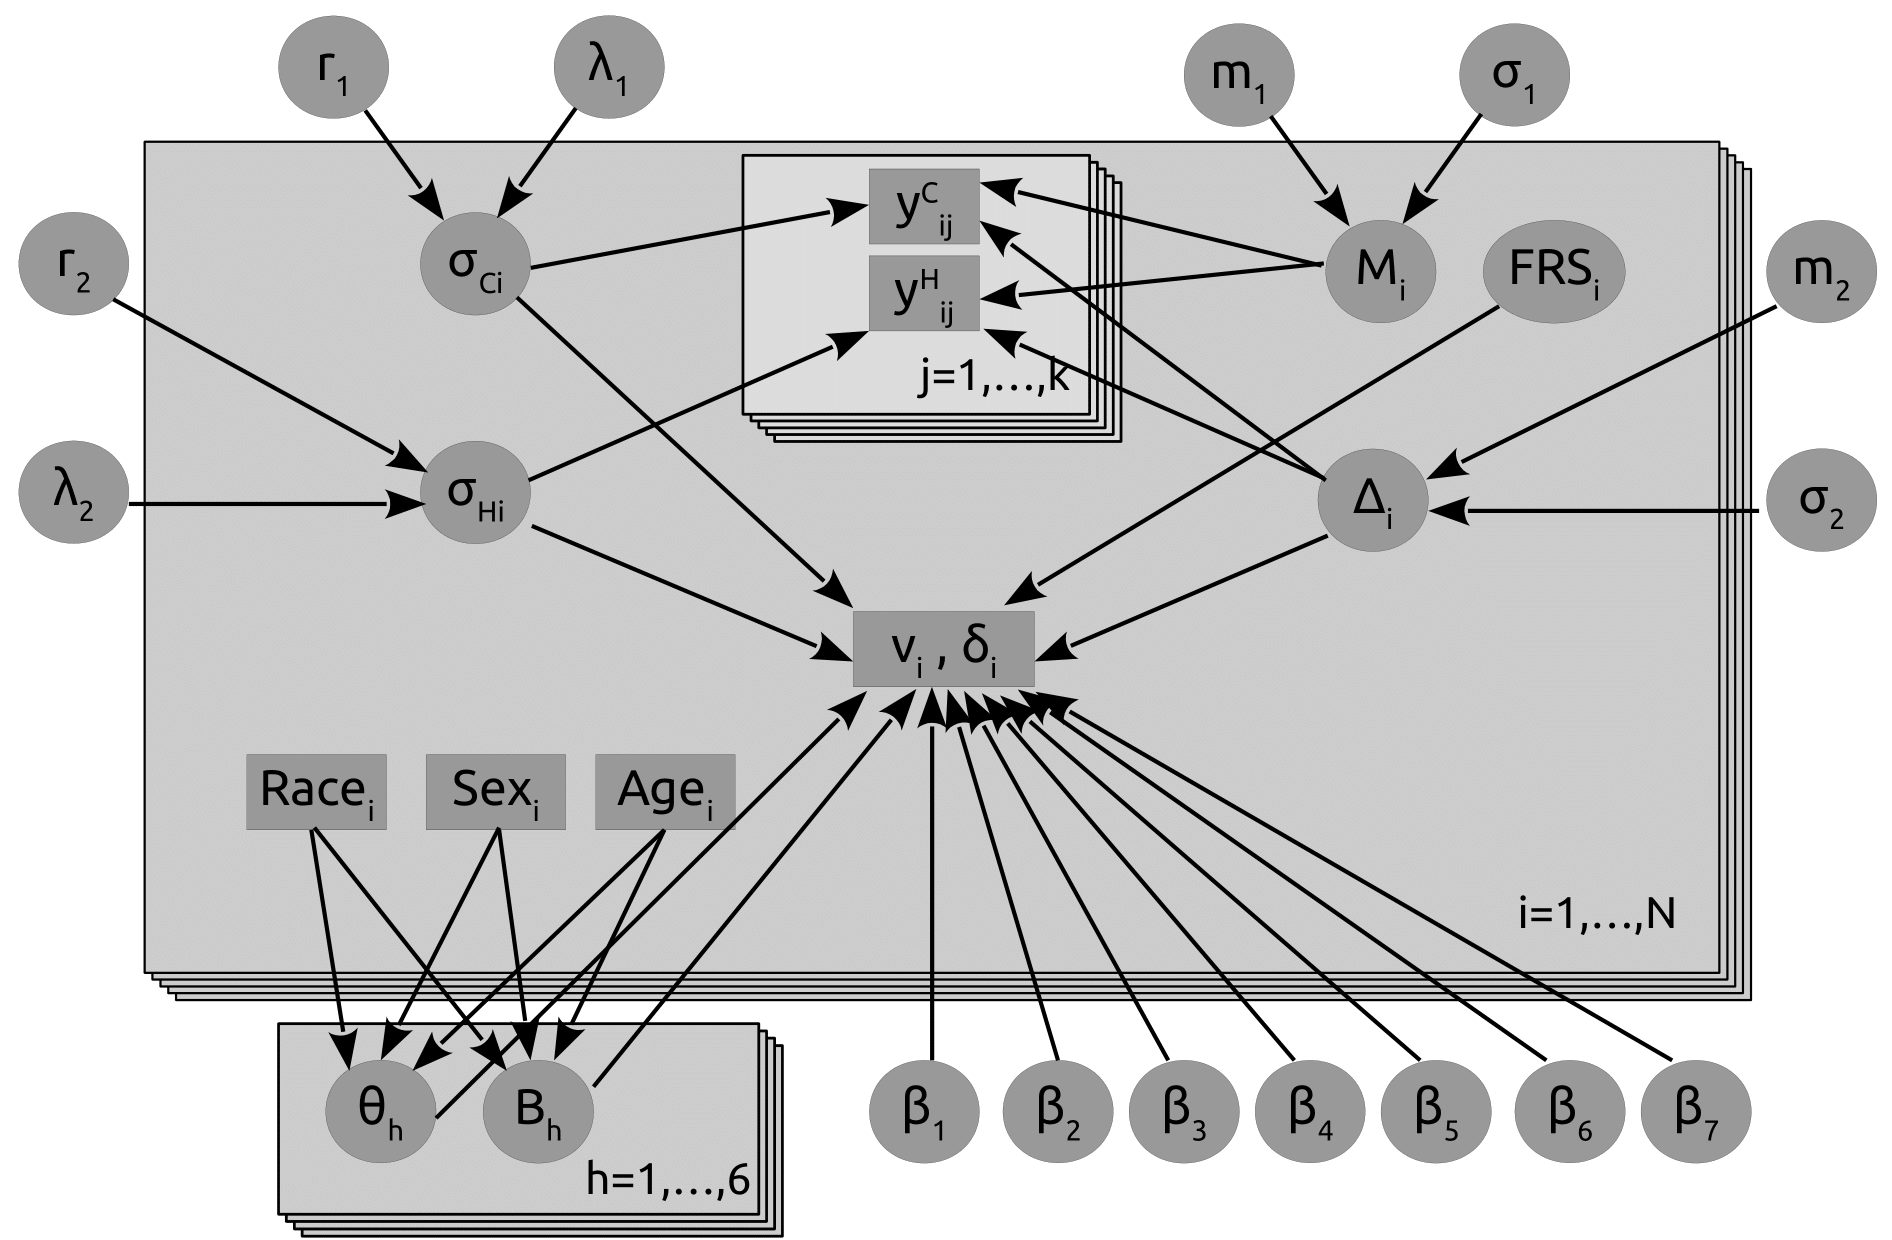
\includegraphics{../DAG_FRS.png}

\hypertarget{methodology}{%
\subsection{Methodology}\label{methodology}}

The methodology for this research can be split into three main sections:
1) calculating the empirical Bayes' parameters, 2) parameterizing the
model using Hamiltonian Monte Carlo (HMC) and 3) re-centering the
variables in the linear predictor equation.

\hypertarget{empirical-bayes-parameters}{%
\subsubsection{Empirical Bayes'
Parameters}\label{empirical-bayes-parameters}}

We begin by assuming \(y_{ij}^l\) observed directly. We estimate by
maximising the partial likelihood on the observations \begin{align*}
  \bar{y}_{i+}&:= \frac{1}{2k} \sum_{j=1}^k y_{ij}^1 + y_{ij}^2,\\
  \bar{y}_{i-}&:= \frac{1}{2k} \sum_{j=1}^k y_{ij}^1 - y_{ij}^2,\\
  s_i^l&:=  \frac{1}{k-1}\sum_{j=1}^k \Bigl( y_{ij}^l - \frac{1}{k} \sum_{j=1}^k y_{ij}^l \Bigr)^2.
\end{align*} Note that \begin{equation}
(k-1)s_i^l \tau_i^l =\sum_{j=1}^k \Bigl( z_{ij}^l - \frac{1}{k} \sum_{j=1}^k z_{ij}^l \Bigr)^2.
\end{equation} where \(z_{ij}^l\) are i.i.d.~standard normal is
independent of \(\tau_i^l\), thus has a chi-squared distribution with
\(k-1\) degrees of freedom --- hence
\(\frac{k-1}{2}\cdot s_i^l\tau_i^l\) is gamma distributed with
parameters \((\frac{k-1}{2},1)\). Since
\(\frac{\alpha}{\theta}\tau_i^l\) is independent of \(s_i^l\tau_i^l\),
with \(\mathrm{Gamma}(\alpha,1)\) distribution, we see that
\(\frac{\theta(k-1)}{2\alpha}s_i^l\) is the ratio of two independent
gamma random variables, hence has beta-prime distribution with
parameters \(\left(\frac{k-1}{2}, \alpha \right)\), so log partial
likelihood \begin{equation}
  \ell_{\operatorname{Beta}}(\alpha,\theta;s^l_\cdot)=n\alpha \log\frac{\alpha}{\theta}+n\log\Gamma\left(\alpha+\frac{k-1}{2}\right)-n\log\Gamma(\alpha)
  + \frac{k-1}{2} \sum_{i=1}^n \log s_i^l -\left(\alpha+\frac{k-1}{2}\right) \sum_{i=1}^n \log \left(s_i^l+\frac\alpha\theta\right).
\end{equation}

The partial Fisher Information has entries \begin{align*}
 -\frac{\partial^2 \ell}{\partial \alpha^2} &= n\psi_1\left(\alpha\right) - n\psi_1\left(\alpha+\frac{k-1}{2}\right)
  - \frac{n}{\alpha} +\sum_{i=1}^n \frac{2\theta s_i^l + \alpha-(k-1)/2}{(\theta s_i^l + \alpha)^2}\\
-\frac{\partial^2 \ell}{\partial \theta^2} &=
   -\frac{n \alpha}{\theta^2} +\frac{\alpha}{\theta^2}\left(\alpha+\frac{k-1}{2}\right)\sum_{i=1}^n \frac{2\theta s_i^l + \alpha}{(\theta s_i^l + \alpha)^2}\\
-\frac{\partial^2 \ell}{\partial \theta\partial\alpha} &= \frac{n}{\theta}-
   \frac1\theta \sum_{i=1}^n \frac{\alpha^2+2\alpha\theta s_i^l+\frac{k-1}{2}\theta s_i^l}{(\theta s_i^l + \alpha)^2}.
\end{align*} where \(\psi_1\) is the trigamma function.

Let \((\hat\alpha^l,\hat\beta^l)\) be the maximum partial likelihood
estimators. Conditioned on \((\tau_i^l)\) we have \begin{align*}
  \bar{y}_{i+}&\sim \mathcal{N}\left(m_M, \sigma^2_M + \frac{1}{4k}\left( \frac{1}{\tau_i^1}+\frac{1}{\tau_i^2}\right)\right),\\
  \bar{y}_{i-}&\sim \mathcal{N}\left(m_\Delta,\sigma^2_\Delta + \frac{1}{4k}\left( \frac{1}{\tau_i^1}+\frac{1}{\tau_i^2}\right)\right).
\end{align*} We would then have MLEs \begin{align*}
  \hat{m}_M&= \frac{1}{n} \sum_{i=1}^n \bar{y}_{i+},\\
  \hat{m}_\Delta&= \frac{1}{n} \sum_{i=1}^n \bar{y}_{i-},
\end{align*} which are approximately normally distributed, with means
\(m_M\) and \(m_\Delta\) respectively, and conditional on \(\tau_i^l\)
standard errors \begin{equation}
  \frac{\sigma_M^2}{n}+\frac{1}{4kn^2} \sum_{i=1}^n (\tau_i^1)^{-1} + (\tau_i^2)^{-1} \quad \text{ and } \quad
  \frac{\sigma_\Delta^2}{n}+\frac{1}{4kn^2} \sum_{i=1}^n (\tau_i^1)^{-1} + (\tau_i^2)^{-1},
\end{equation} which we may approximate --- with error on the order of
\(n^{-3/2}\) --- replacing the mean of \((\tau_i^l)^{-1}\) by its
expected value \(\beta^l/(\alpha^l-1)\) to obtain \begin{align*}
  \mathrm{Var}(\hat{m}_M) &\approx \frac{\sigma_M^2}{n}+\frac{1}{4kn}\left( \frac{\beta^1}{\alpha^1-1}+ \frac{\beta^2}{\alpha^2-1}\right) \\
  \mathrm{Var}(\hat{m}_\Delta) &\approx \frac{\sigma_\Delta^2}{n}+\frac{1}{4kn}\left( \frac{\beta^1}{\alpha^1-1}+ \frac{\beta^2}{\alpha^2-1}\right) 
\end{align*} Finally, conditioned on the \(\tau_i^l\) we have that the
random variables \(\bar{y}_{i+}\) are normal with variance
\begin{equation}
  \sigma_M^2+\frac{1}{4k}\left((\tau_i^1)^{-1} + (\tau_i^1)^{-1} \right),
\end{equation} so the unconditional variance is the expected value, or
\begin{equation}
  \sigma_M^2+\frac{1}{4k}\left(\frac{\beta^1}{\alpha^1-1}+ \frac{\beta^2}{\alpha^2-1} \right).
\end{equation} This yields the estimators \begin{align*}
  \hat\sigma_M^2 &=\frac{1}{n-1}\sum_{i=1}^n\left(\bar{y}_{i+}-n^{-1}\sum_{i=1}^n y_{i+}\right)^2 - \frac{1}{4k}\left(\frac{\hat\beta^1}{\hat\alpha^1-1}+ \frac{\hat\beta^2}{\hat\alpha^2-1} \right),\\
  \hat\sigma_\Delta^2 &=\frac{1}{n-1}\sum_{i=1}^n\left(\bar{y}_{i-}-n^{-1}\sum_{i=1}^n y_{i-}\right)^2 - \frac{1}{4k}\left(\frac{\hat\beta^1}{\hat\alpha^1-1}+ \frac{\hat\beta^2}{\hat\alpha^2-1} \right).
\end{align*} Using the delta method, and the fact that we see that the
variance of \(\hat\beta/(\hat\alpha-1)\) is approximately
\begin{equation}
  \frac{\sigma_\beta^2}{(\hat\alpha-1)^2} + \frac{\hat\beta^2\sigma_\alpha^2}{(\hat\alpha-1)^4},
\end{equation} where \(\sigma_\alpha\) and \(\sigma_\beta\) are the
standard errors for \(\hat\alpha\) and \(\hat\beta\) respectively, so
the standard errors for \(\hat\sigma_M^2\) and \(\hat\sigma_\Delta^2\)
are approximately \begin{align*}
  \operatorname{SE}\left(\hat\sigma_M^2\right)&\approx \frac{1}{2k}\Bigl(\frac{8k^2\hat\sigma_M^2}{n} + \frac{\sigma_\beta^2}{(\hat\alpha^1-1)^2} + \frac{(\hat\beta^1)^2\sigma_\alpha^2}{(\hat\alpha^1-1)^4} + \frac{\sigma_\beta^2}{(\hat\alpha^2-1)^2} + \frac{(\hat\beta^2)^2\sigma_\alpha^2}{(\hat\alpha^2-1)^4} \Bigr)^{1/2},\\
  \operatorname{SE}\left(\hat\sigma_\Delta^2\right)&\approx \frac{1}{2k}\Bigl(\frac{8k^2\hat\sigma_\Delta^2}{n} + \frac{\sigma_\beta^2}{(\hat\alpha^1-1)^2} + \frac{(\hat\beta^1)^2\sigma_\alpha^2}{(\hat\alpha^1-1)^4} + \frac{\sigma_\beta^2}{(\hat\alpha^2-1)^2} + \frac{(\hat\beta^2)^2\sigma_\alpha^2}{(\hat\alpha^2-1)^4} \Bigr)^{1/2}
\end{align*}

For a parameter like \(\alpha\) we estimate the variance of
\(\hat\alpha\) by \newcommand{\E}{\mathbb{E}}
\renewcommand{\P}{\mathbb{P}} \begin{equation}
  \mathrm{Var}(\hat\alpha) = \mathbb{E}\bigl[ \mathrm{Var}\left(\hat\alpha\, |\, I\right)\bigr] + \mathrm{Var}\left(\mathbb{E} \left[ \hat\alpha\, |\, I \right]\right).
\end{equation} Here \(I\) represents the randomly imputed fractional
part. We can estimate the first term by averaging the estimated variance
(from Fisher Information) over all random imputations. We estimate the
second term by the variance of the \(\alpha\) estimates over
imputations. Note that this is not quite right, since what we really
want the variance of is \(\alpha_0(I)\) --- effectively, the `true'
parameter consistent with the imputation. This is a plug-in estimate, as
is the Fisher Information estimate of the variance.

To computing the residuals, we define the deviance for an individual
\(i\) with observations \((Y_i)\) given the hyperparameters
\(h=(m_M,m_\Delta,\sigma^2_M,\sigma^2_\Delta,\alpha^H,\theta^H,\alpha^C,\theta^C)\)
\begin{equation}
  D= \sum_{i=1}^n \log \mathbb{P}\left\{ \mathbf{Y}_{i}\,|\, \text{hyperparameters}=h\right\}.
\end{equation} \newcommand{\wtb}{\widetilde\mathbf} Since the
\(\mathbf{Y}_i\) are independent conditioned on \(h\), \begin{align*}
D&= \sum_{i=1}^n \log \mathbb{E}_h\left[ \mathbb{P}\left\{ \mathbf{Y}_i \, |\, M_i,\Delta_i,\tau_i^{C},\tau_i^H \right\} \right]\\
    &\approx \sum_{i=1}^n \log \frac1R\sum_{r=1}^R \left[ \mathbb{P}\left\{ \mathbf{Y}_i \, |\, M_{i,r},\Delta_{i,r},\tau_{i,r}^{C},\tau_{i,r}^{H} \right\}\right] \frac{\pi_h(M_{i,r},\Delta_{i,r},\tau_{i,r}^{C},\tau_{i,r}^{H} )}{q(M_{i,r},\Delta_{i,r},\tau_{i,r}^{C},\tau_{i,r}^{H} \, | \, h,\, \mathbf{Y}_i)},
\end{align*} where
\((M_{i,r},\Delta_{i,r},\tau_{i,r}^{C},\tau_{i,r}^{H})\) are independent
samples from a distribution \(q\) that may depend on \(\mathbf{Y}_i\)
and \(h\), and \(\pi_h\) is the true density of those individual
parameters given hyperparameters \(h\).

\hypertarget{hamiltonian-monte-carlo-hmc}{%
\subsubsection{Hamiltonian Monte Carlo
(HMC)}\label{hamiltonian-monte-carlo-hmc}}

The model, as described in the article, is a Bayesian hierarchical
model. In order to parameterize such an intricate model, traditional
Maximum Likelihood Estimation methods can no longer be applied.
Therefore, we apply the Hamiltonian Monte Carlo (HMC) method. HMC is a
form of Markov Chain Monte Carlo methods, which samples potential
parameter space values of the model, then calculates directly the
likelihood function based on that choice of parameters. The derivative
of the likelihood function, \(\phi\), guides parameter space exploration
in \(\theta\) towards the modal value of the joint posterior
distribution. This method is ideal for complicated, non-Gaussian
distribution forms. The three steps of HMC are:

\begin{enumerate}
\item Draw a sample of the derivative $\phi$ using the posterior distribution of $\phi$, which is the same as its prior.
\item Update the values of $\theta^*$ and $\phi^*$ using
  \begin{equation}
    \theta^*\leftarrow \theta+\epsilon M^{-1}\phi,
  \end{equation}
  and
  \begin{equation}
    \phi\leftarrow \phi+\epsilon\frac{1}{2}\frac{d\log\{p(\theta|y)\}}{d\theta},
  \end{equation}
where $M$ is the jacobian of the parameters. This can be set to a diagonal matrix for no correlation between parameters, and is pointwise updated throughout the calculation. This is the leapfrog method, whereby $\epsilon$ dictates the scale size of the step to ensure convergence on the correct point is made, and L is the number of steps to be `leaped'.
\item Compute the rejection parameter:
  \begin{equation}
    r=\frac{p(\theta^*|y)p(\phi^*)}{p(\theta^{t-1}|y)p(\phi^{t-1})}
  \end{equation}
\item Set $\theta^t$ to $\theta^*$ with probability $\min\{1,r\}$, or otherwise keep $\theta^{t-1}$.
\end{enumerate}

The tuning parameters \(\epsilon\) and L should be chosen according to a
desired acceptance rate. The No-U-Turn Sampler of Stan automates the
calculation of these tuning parameters. A more detailed overview of HMC
and the NUTS algorithm integrated into the Stan package, see \emph{`The
No-U-Turn Sampler: Adaptively Setting Path Lengths in Hamiltonian Monte
Carlo'} by M. Hoffman and A. Gelman, Journal of Machine Learning
Research, 15, 1351-1381 (2014).

\hypertarget{centering-the-linear-predictor}{%
\subsubsection{Centering the Linear
Predictor}\label{centering-the-linear-predictor}}

During the MCMC simulations, the centering values play a non-negligible
role in shaping the model parameterization. If the centering parameters
are held constant throughout all of the MCMC simulations, then the
equation
\(\sum_i^N \exp{(\boldsymbol{\beta}\cdot(\boldsymbol{X}-\hat{X}))}=0\)
is no longer guaranteed. However, automatically defining the centering
values based on the model parameters sampled at the current MCMC
iteration is not advisable as it can lead to poor parameter convergence
as it modifies the likelihood function at every MCMC iteration.
Therefore, we iterate the MCMC algorithm multiple times. At every
iteration, we recalculate the centering parameters to satisfy the
requirement that the average of the linear predictor term going to zero,
based on the posterior distributions of the previous MCMC simulation.
This iteration is carried out until the centering parameters converge.
Convergence is defined by optimising on two factors. The first is that
the sum of the linear predictor term across all MCMC samples needs to
tend to negligible values (we define this as the average difference
being less than \(10^{-7}\)), see figure A.3 (below). The second
convergence criteria is that the average Root Mean-Squared Error (RMSE)
of the model predictions on the survival outcomes in the MCMC
simulations needs to also decrease towards zero, see figure A.3 (top).
For the second criteria, we stopped the simulations when either the
difference in the RMSE stopped decreasing (below a threshold of
\(1\%\)), or the RMSE value was less than 20. Illustration of the
convergence is shown in figure A.3.

\hypertarget{code-description}{%
\subsection{Code Description}\label{code-description}}

The code can be found at \url{https://github.com/hamishwp/Nhanes2021}.
The numerical code has been built in multiple stages. Below, we explain
the principal files required to replicate the entire analysis presented
in the article. There are 5 main groups for the code:

\begin{enumerate}
\def\labelenumi{\arabic{enumi}.}
\tightlist
\item
  Data cleaning scripts
\item
  Main file
\item
  Stan files for HMC
\item
  Centering recalculation scripts
\item
  Post-processing analysis
\end{enumerate}

We provide a brief description of each of these below.

\hypertarget{data-cleaning}{%
\subsubsection{Data Cleaning}\label{data-cleaning}}

This is found in the file \texttt{Dataclean2021.R}. Provided the raw
NHANES dataset (in CSV format), it extracts all the data required for
the simulations, and stores it in a structure that can be directly read
in to the main file (\texttt{MCMC\_DiasSyst\_v3.R}) of this research.

\hypertarget{main}{%
\subsubsection{Main}\label{main}}

The main file is \texttt{MCMC\_DiasSyst\_v3.R}. It reads in the cleaned
NHANES data, the specific choice of simulation parameters (for example,
whether to use the FRS number or mean systolic \& diastolic blood
pressure), and runs the correct RStan scripts for that specific
selection of simulation parameters. This script is intended for use on
computing clusters.

\hypertarget{stan}{%
\subsubsection{Stan}\label{stan}}

There are eight Stan files:
\texttt{mystanmodel\_DS\_sigma\_v2\_autopred.stan},
\texttt{mystanmodel\_DS\_tau\_v2\_autopred.stan},
\texttt{mystanmodelFRS\_DS\_sigma\_v2\_autopred.stan},
\texttt{mystanmodelFRS\_DS\_tau\_v2\_autopred.stan},
\texttt{mystanmodel\_DS\_sigma\_v2.stan},
\texttt{mystanmodel\_DS\_tau\_v2.stan},
\texttt{mystanmodelFRS\_DS\_sigma\_v2.stan},
\texttt{mystanmodelFRS\_DS\_tau\_v2.stan}. These correspond to the
following alternative simulation parameters:

\begin{itemize}
\tightlist
\item
  For the blood-pressure variability, choosing to use the
  standard-deviation \(\sigma\) or the precision \(\tau=1/\sigma\){]}\}
\item
  Using the FRS score or the mean diastolic and systolic blood pressure
  as a covariate in the analysis
\item
  Whether the centering parameters, \(\hat{X}\), in the linear predictor
  term are automatically calculated to satisfy
  \(\sum_i^N \exp{(\boldsymbol{\beta}\cdot(\boldsymbol{X}-\hat{X}))}=0\)
  for every MCMC iteration, or whether the centering is held constant
  across all iterations
\end{itemize}

\hypertarget{centering}{%
\subsubsection{Centering}\label{centering}}

The centering of the linear predictors, which is required as input to
every MCMC simulation iteration, is recalculated in the files
\texttt{AutoPred\_Recalc.R} and \texttt{ManPred\_Recalc.R}. This is then
provided to the Main script, \texttt{MCMC\_DiasSyst\_v3.R}, which
provides these centering values to the Stan code for the MCMC
simulations.

\#\#\#Post-processing The post-processing script is called
\texttt{PostProcessing.R}, which heavily relies on the
\texttt{Functions.R} script which contains all the necessary functions
to analyse the data. The post-processing script generates many useful
plots of the MCMC posterior distribution for the user, including Bayes'
factors, violin plots of the normalised beta and gompertz posteriors,
and more.

\hypertarget{results}{%
\subsection{Results}\label{results}}

In this section, we add some additional detail to the results section
covered in the article. Extra information is given to explain how
convergence of the simulations was ensured, and to also include more
visualisations of the converged model parameterizations. The authors
feel that this is particularly useful to provide confidence in the model
parameterization and the predictions.

\hypertarget{convergence-of-simulations}{%
\subsubsection{Convergence of
Simulations}\label{convergence-of-simulations}}

Convergence of the simulations required to parameterize the model
presented in this work is required for the MCMC simulations performed by
Stan, as well as convergence in the centering values that requires
repeating the Stan calculations several times. Convergence of the latter
is shown in figure A.3. The upper plot in figure A.3 illustrates
convergence in the average Root Mean-Squared Error (RMSE) of the model
predictions on the survival outcomes in the MCMC simulations. The lower
plot in figure A.3 illustrates convergence in the average sum of the
linear predictor terms over all MCMC chain iterations.

\begin{figure}
\centering
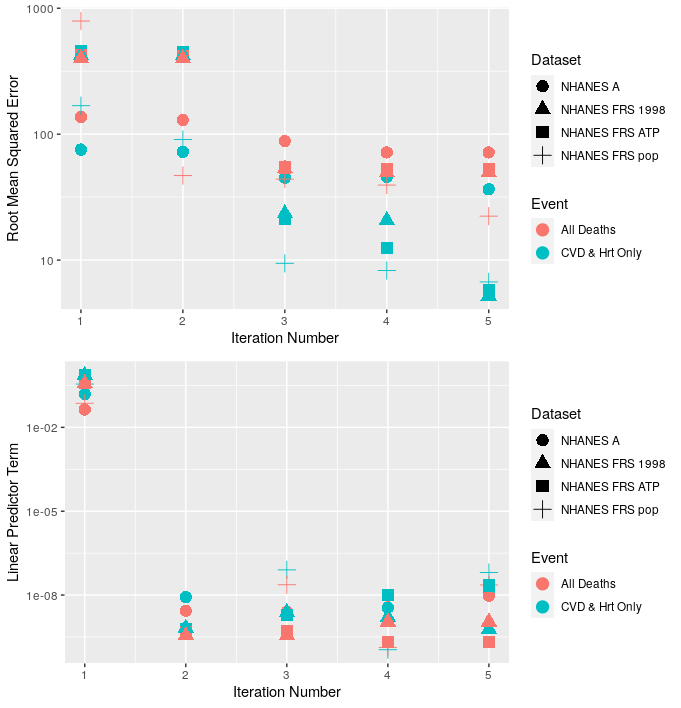
\includegraphics{../Plots/xhat/RMSE-Linpred_Convergence.png}
\caption{Figure A.3: illustration of the convergence of the centering
parameters of the model}
\end{figure}

With respect to convergence of the MCMC simulations, defining
convergence first involves discarding the burn-in period of the
simulations. When the time-evolution marker chain has a large number of
samples, sequence thinning is used to reduce the amount of data storage
- after convergence, take only the kth value of the simulations (after
having discarded the burn-in phase values) and discard the rest. One
measure of convergence is to bin similar markers and check that for each
bin, the variation of the individual marker movement over a few time
steps is larger than the variation of the ensemble markers in-between
one-another. Other methods of convergence are stationarity and mixing.
The former occurs by ensuring that the gradients of movements in the
chains in time are in the same direction, the latter ensures that the
amplitude of the movements in the chains are similar. To calculate the
mixing and stationarity, one can do the following:

\begin{itemize}
\item Take the proposedly converged marker population, where there are N markers in total each of index length $\tau$ (thus of total physical time quantity $t\tau$). Split it k times, where k is a common denominator of $\tau$.
\item Now you have $kN$ MCMC chains each of length $|\tau/k|$
\item For the marker $\psi_{ij}$ with i and j the chain length (time) and marker number indices respectively, then the mean marker value over the chain length (time) is
  \begin{equation}
    \bar{\psi}_{|,j}=\frac{k}{\tau}\sum_{i=1}^{\tau/k}\psi_{ij}
  \end{equation}
  and the total average quantity of $\psi$ over all markers, over all chain lengths is therefore
  \begin{equation}
    \bar{\psi}_{||}=\frac{1}{kN}\sum_{j=1}^{kN}\bar{\psi}_{|j}
  \end{equation}  
\item Stationarity: compare the inter-marker variance (between sequence B):
  \begin{equation}
    B = \frac{\tau}{k(kN-1)}\sum_{j=1}^{kN}(\bar{\psi}_{|,j}-\bar{\psi}_{||})^2
  \end{equation}
\item Mixing: compare the variance along each markers chain length (within-sequence W):
  \begin{equation}
    W = \frac{1}{n(\tau-k)}\sum_{j=1}^{kN}\sum_{i=1}^{\tau/k}(\psi_{i,j}-\bar{\psi}_{|j})^2
  \end{equation}
\item Therefore, to estimate the marginal posterior variance of $p(\psi|y)$, then we use a weighted average
  \begin{equation}
    \hat{\text{Var}}^+(\psi|y)=\frac{\tau-k}{N}W+\frac{1}{Nk}B
  \end{equation}
  Note that this quantity overestimates the marginal posterior variance, but it is unbiased under stationarity: this can be used to infer convergence. When the varation in
  \begin{equation}
    \hat{R}=\sqrt{\frac{\hat{\text{Var}}^+(\psi|y)}{W}}
  \end{equation}
  should approach close to 1 for converged simulations.
\end{itemize}

Another convergence parameter is the number of effective independent
marker draws. Upon convergence, the time evolution of each marker should
be uncorrelated and independent to previous time steps. To find the
average time-correlation over all particles, we use the variogram
\(V_t\): \begin{equation}
  V_t=\frac{1}{Nk(\tau/k-\tilde{t})}\sum_{j=1}^{kN}\sum_{i=1}^{\tau/k}(\psi_{i,j}-\psi_{i-\tilde{t},j})^2,
\end{equation} where \(\tilde{t}\in 1,2,...,\tau/k\) is a time index.
Then we get the time-correlations: \begin{equation}
  \hat{\rho}_t=1-\frac{V_t}{2\hat{\text{Var}}^+}
\end{equation} This comes from the expectation of the variance
\(E[(\psi_i-\psi_{i-t})^2]=2(1-\rho_t)\text{Var}(\psi)\). This can be
used to infer the effective number of independent marker draws:
\begin{equation}
  \hat{n}_{eff}=\frac{mn}{1+2\sum_{\tilde{t}=1}^T\hat{\rho}_t}
\end{equation} Where T is the index at which the sum of the
autocorrelation estimates \(\hat{\rho}_{t'}+\hat{\rho}_{t'+1}\) is
negative. As a general guide, we should have \(\hat{n}_{eff}\sim 10N/k\)
effective independent marker draws and that \(\hat{R}\to 1\sim 1.1\). In
this research, we continued running the MCMC simulations until these two
criteria were met (and went beyond: \(\hat{R}<1.05\) for all parameters
in all models and that \(\hat{n}_{eff}>750\) for all parameters in all
models).

\hypertarget{results---model-parameterization}{%
\subsubsection{Results - Model
Parameterization}\label{results---model-parameterization}}

We remind the reader of the list of numbers of the different models
explored in this research, provided in list \ref{runnums}. The authors
will use the numbers in the list, referred to as the run number, in the
following plots. One of the most important set of parameters of the
model is the vector \(\beta\) of covariates in the Cox' proportional
hazards model. When the \(\beta\) vector is normalised, the larger (in
absolute terms) the value of \(\beta\), the larger the correlation
between that specific covariate and the risk of mortality. Positive
values of \(\beta\) imply a higher risk of mortality, and the inverse
for negative values of \(\beta\). As we can see from the violin plots of
the MCMC posterior samples of the \(\beta\) parameters in figure A.4,
the parameter that correlated the highest with both the mortality risk
of CVD or heart attack and for all mortalities, in absolute terms, was
the 1998 version of the FRS score, shown in the top-right plot under run
numbers 7 and 8. The FRS-1998 score correlated, on average over all the
MCMC iterations, approximately \(25\%\) more with mortality risk of CVD
and heart attack than the (more recently developed) FRS ATP III score. A
similar, but slightly weaker, correlation was found between the two FSR
scores for all mortality-based risk. The middle-left plot shows that the
mean diastolic blood pressure acts to decrease mortality risk. Finally,
the influence of the longer-term difference in the mean blood pressure,
displayed in the top-left and top-middle plots, is also shown to
increase mortality risk across all run numbers. The influence of the
blood-pressure variability on mortality is illustrated to not be
consistent across simulations, whereby the statistical significance of
the effect is lower than for the other parameters in the linear
predictor term.

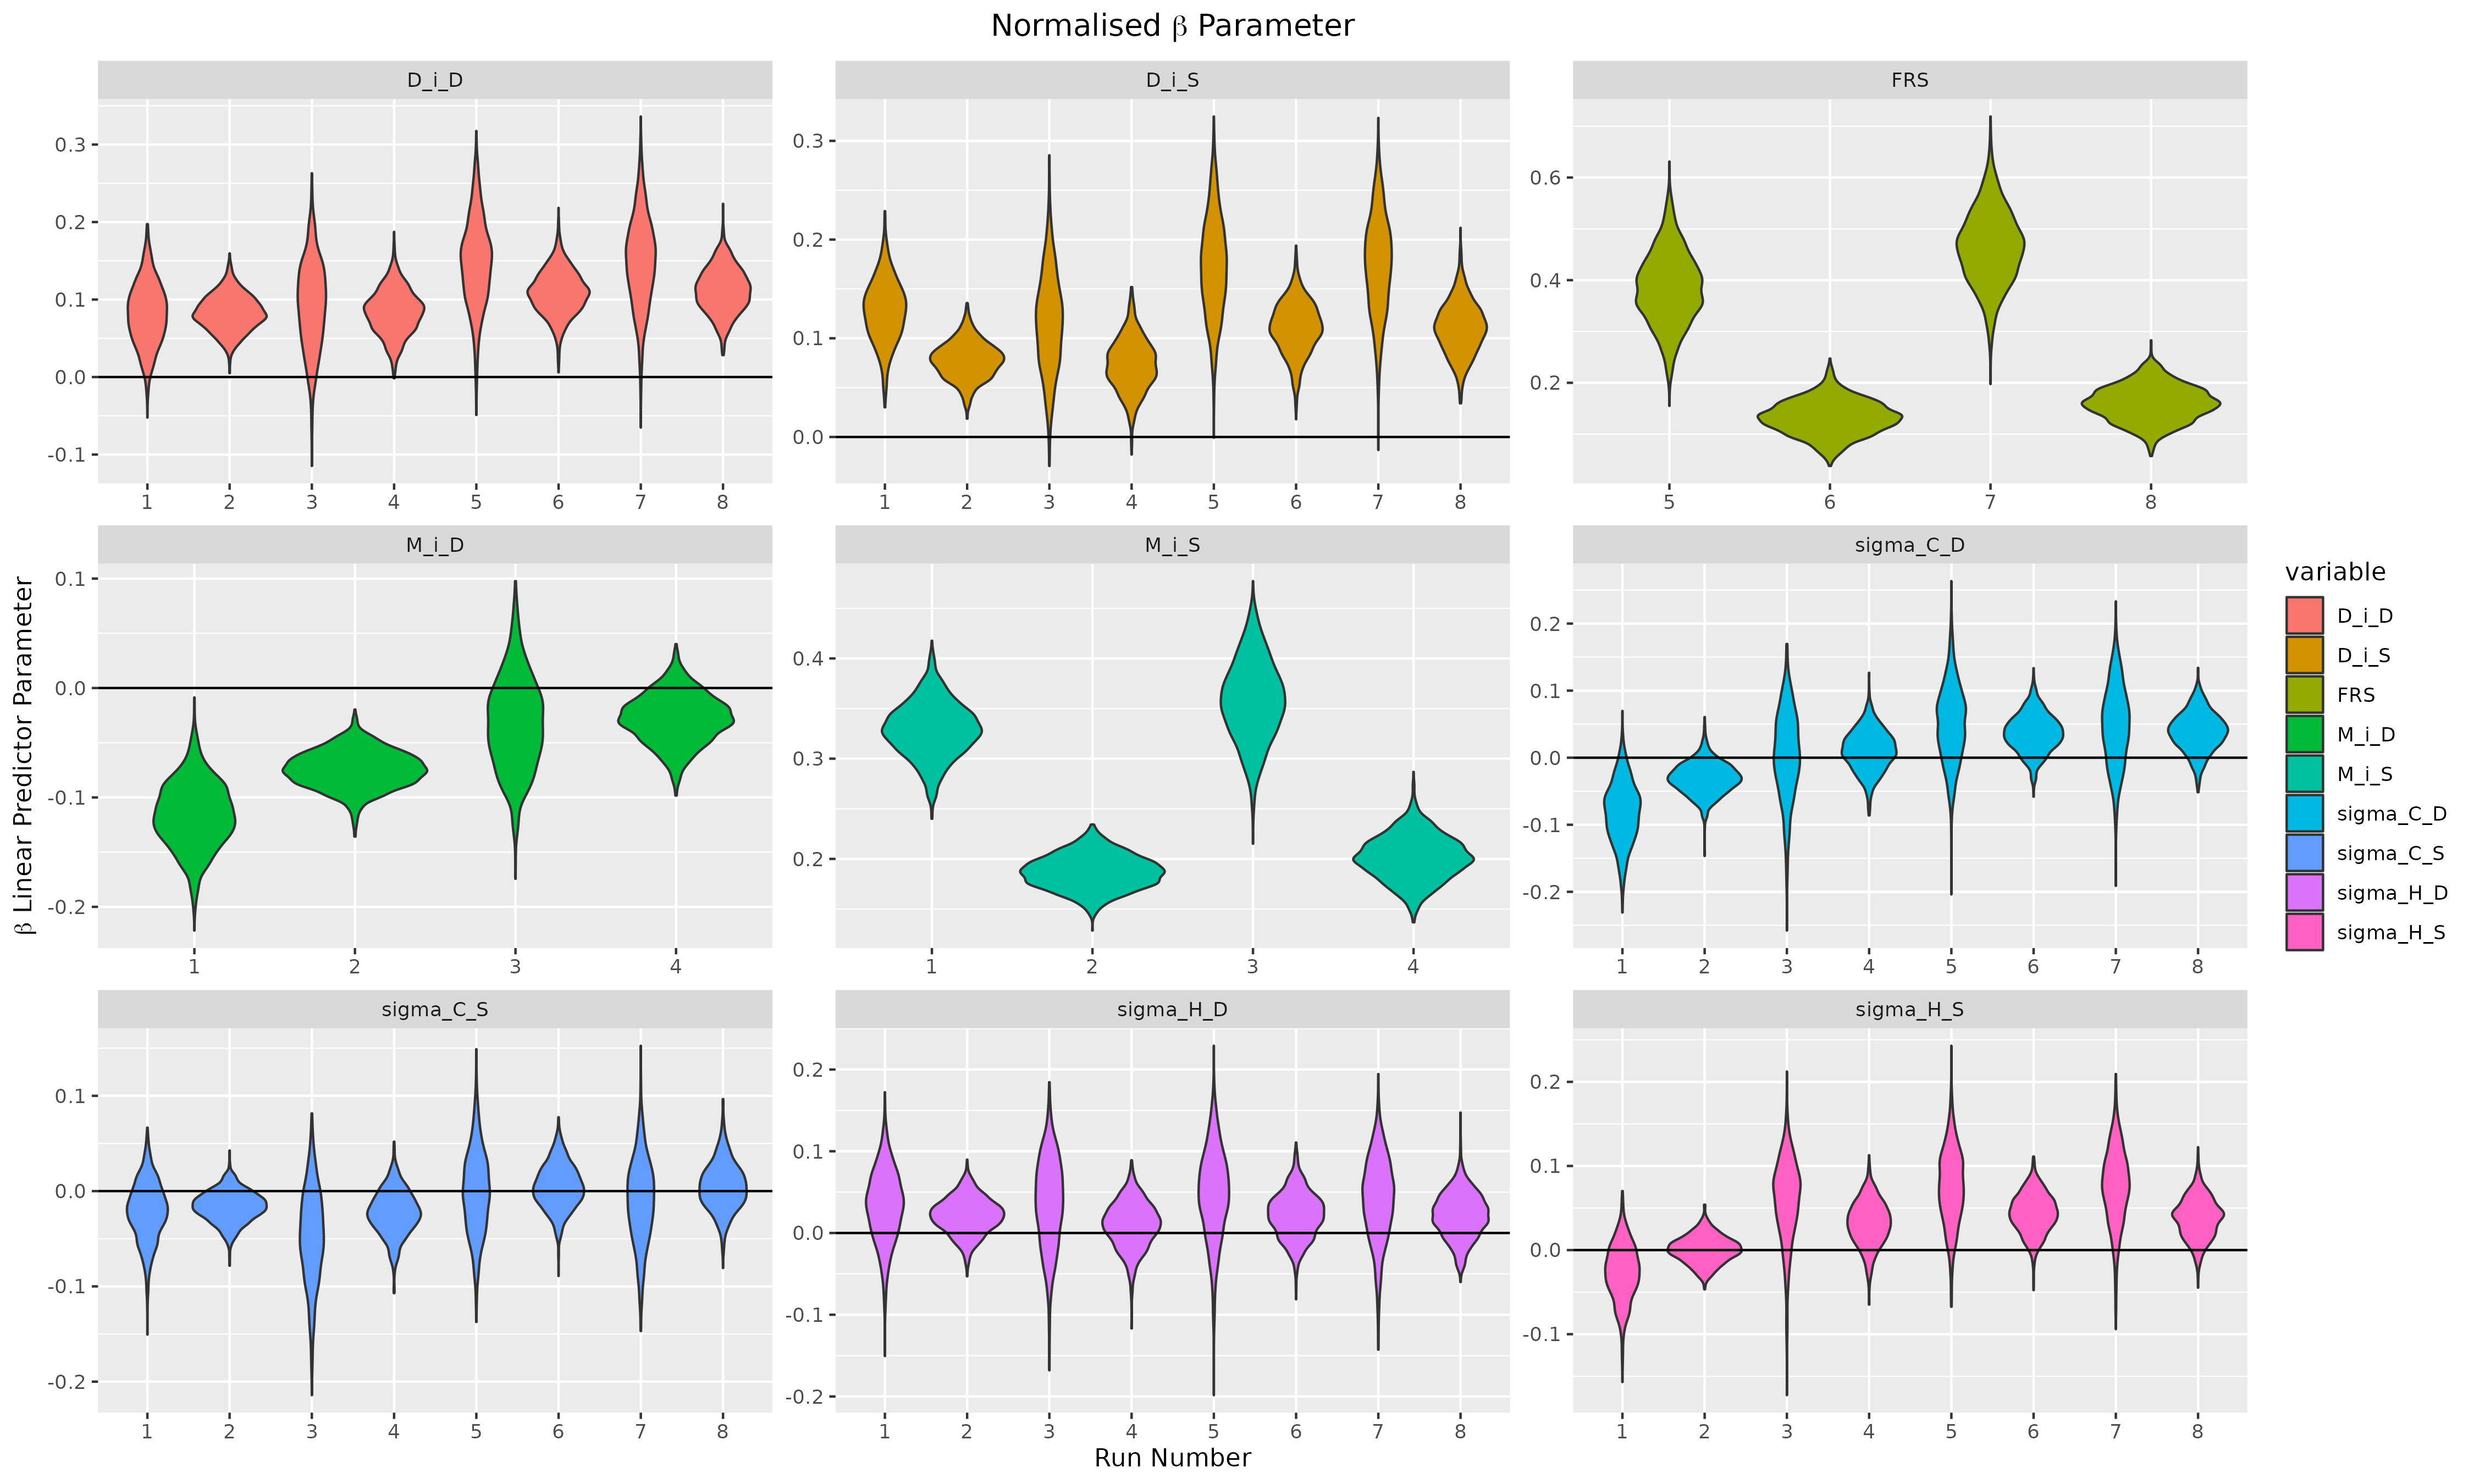
\includegraphics{../Plots/beta/Beta_parameter_normalised.png} With
respect to the time-independent Gompertz parameter, described using
\(B\) in this article, the results between all models that simulate CVD
and heart attack mortality risk, and all the models that simulation
all-cause mortality risk are consistent with one-another. This is
illustrated by the similarity between plots on the left hand side and
the right hand side of figure A.5. The consistency appears across sex
assigned at birth and race.

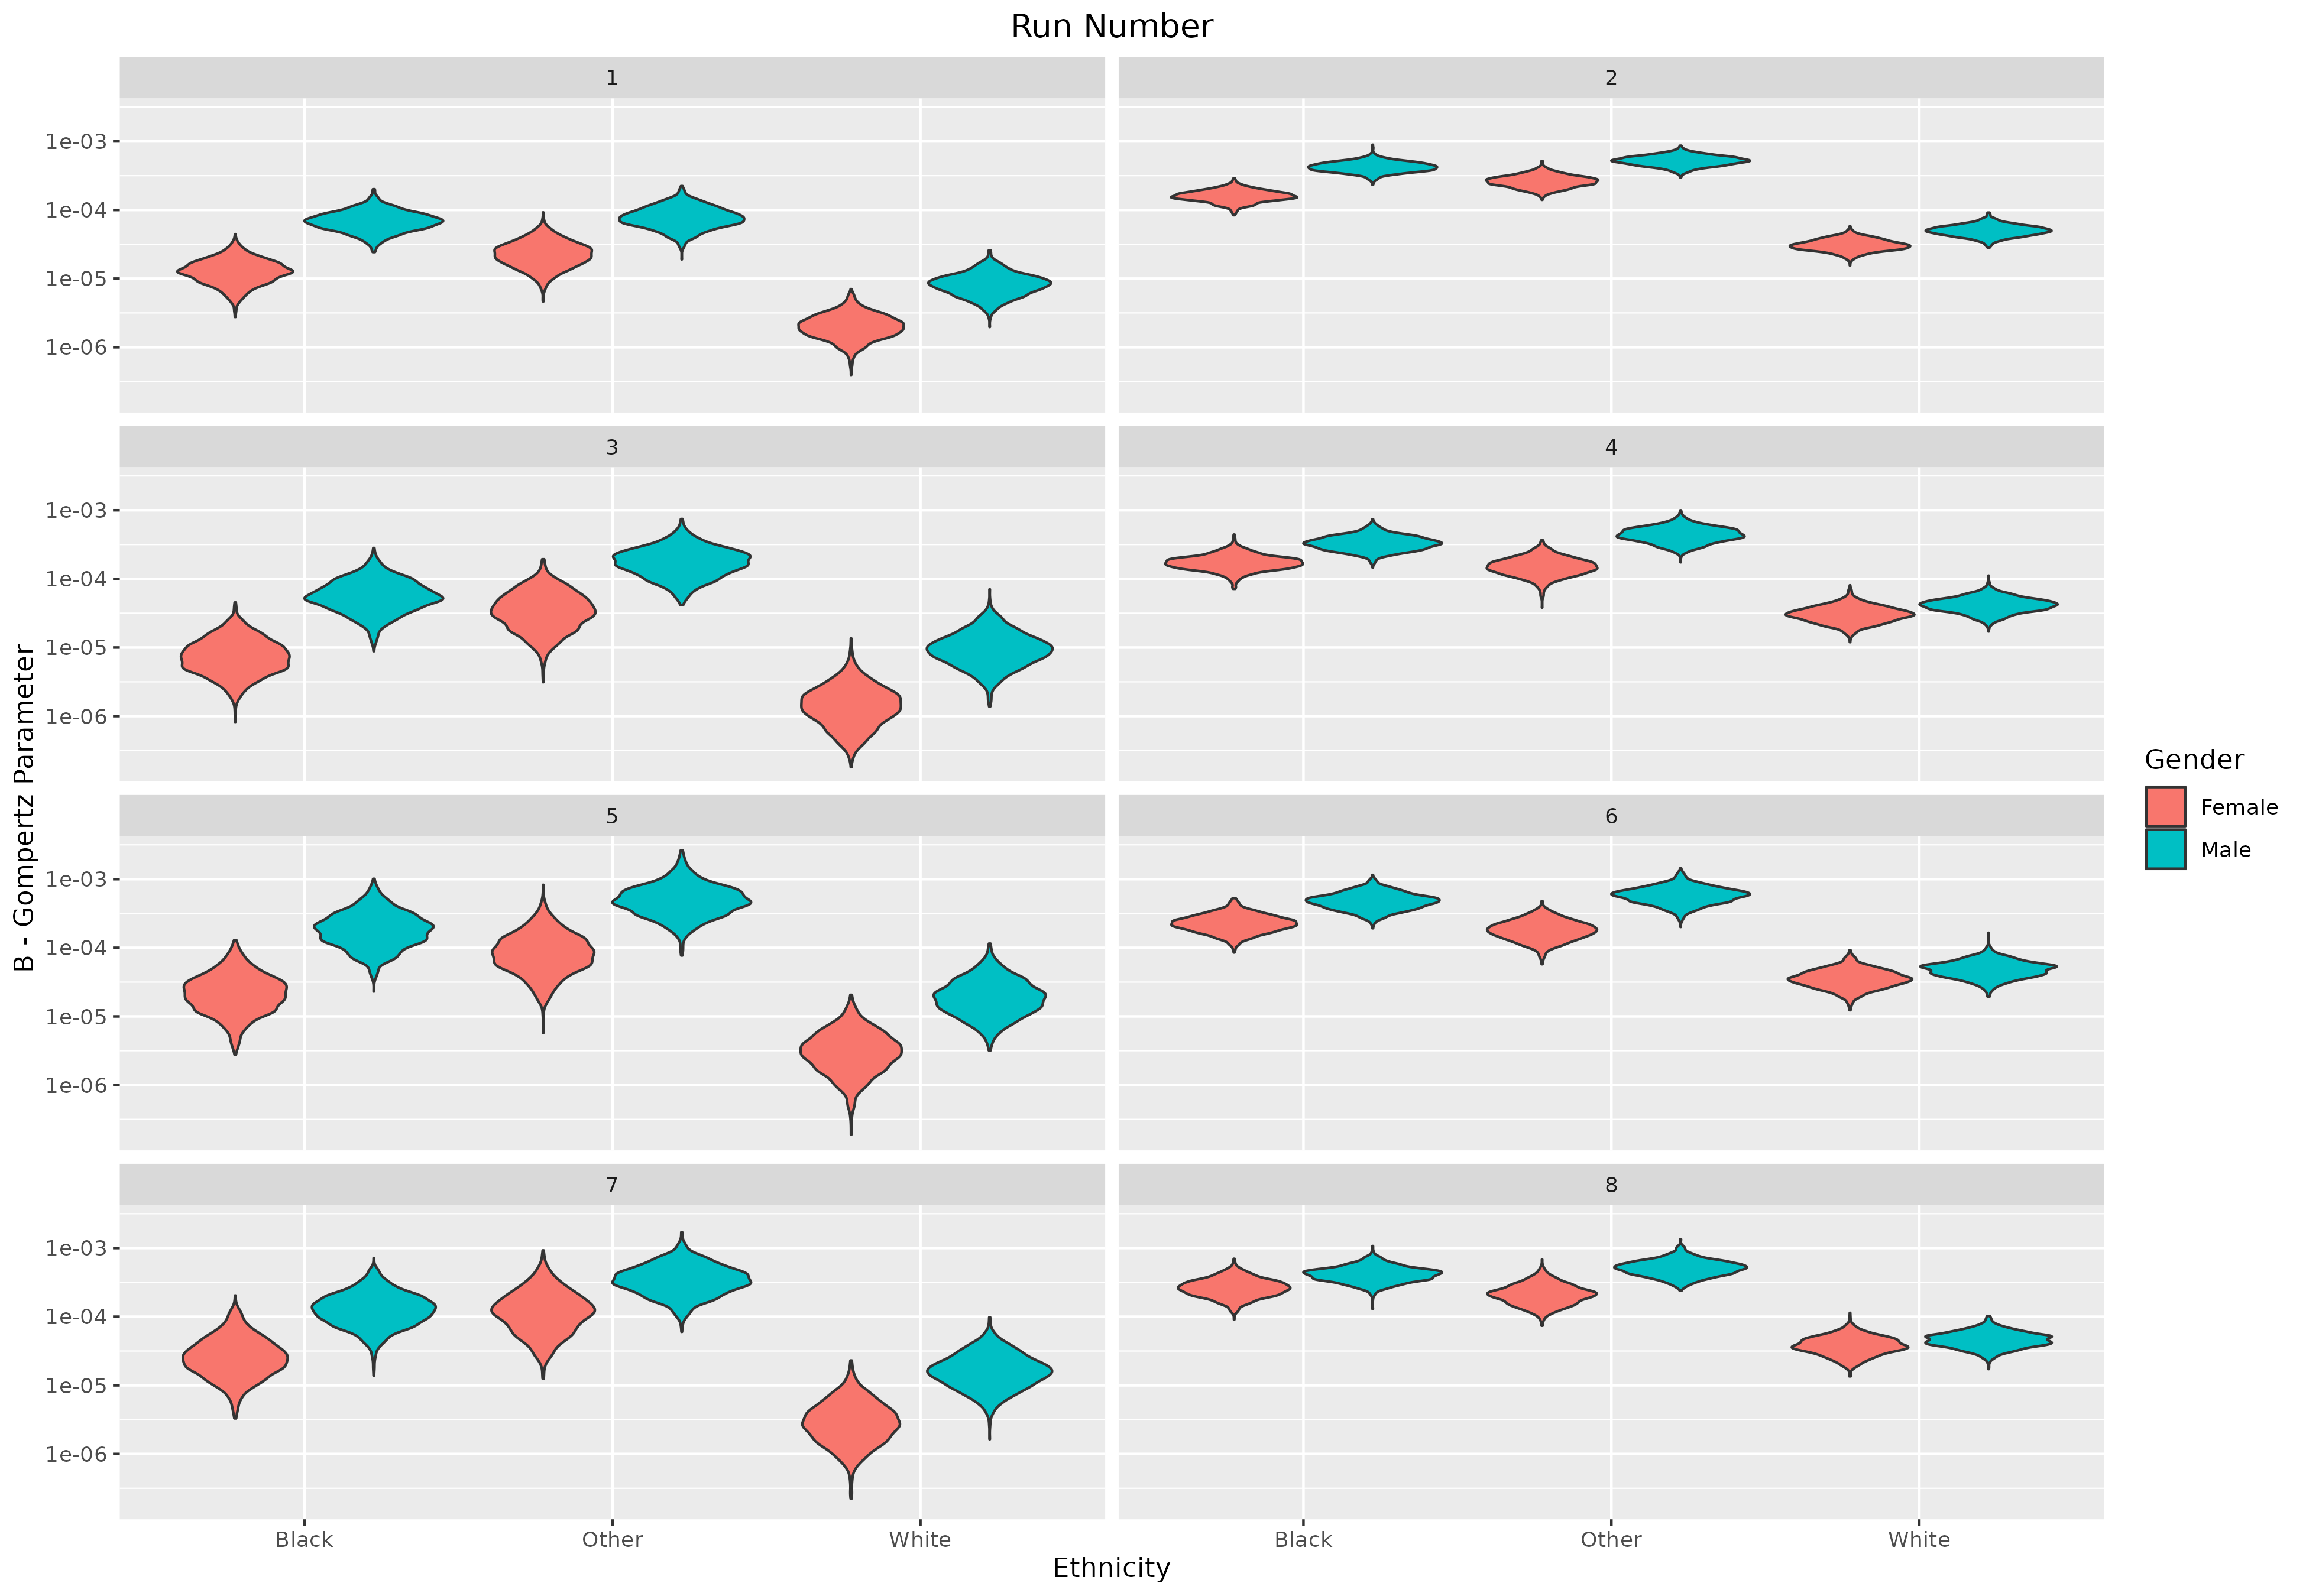
\includegraphics{../Plots/gompertz/B_parameter.png} Figure A.6 reflects
the same level of consistency for the Gompertz parameter that influences
the temporal evolution of the mortality risk. It is worth noting that
both figures A.5 and A.6 have inverse trends between the values of B and
theta for each demographic group. This makes it difficult to imagine,
based on these two plots, what the mortality risk is at different ages
across demographics, yet it is evident that the form of the change in
the mortality risk curve in time is different for each demographic
group. Women are observed to have lower initial values of risk, but
mortality risk later in life begins to increase much faster than for
men. Additionally, hispanic populations are shown to have a larger
initial mortality risk than black populations who are shown to have a
larger initial mortality risk than white populations in the USA.
However, mortality risk increases at a faster rate for white populations
than for black populations, for which it increases faster than hispanic
populations in the USA.

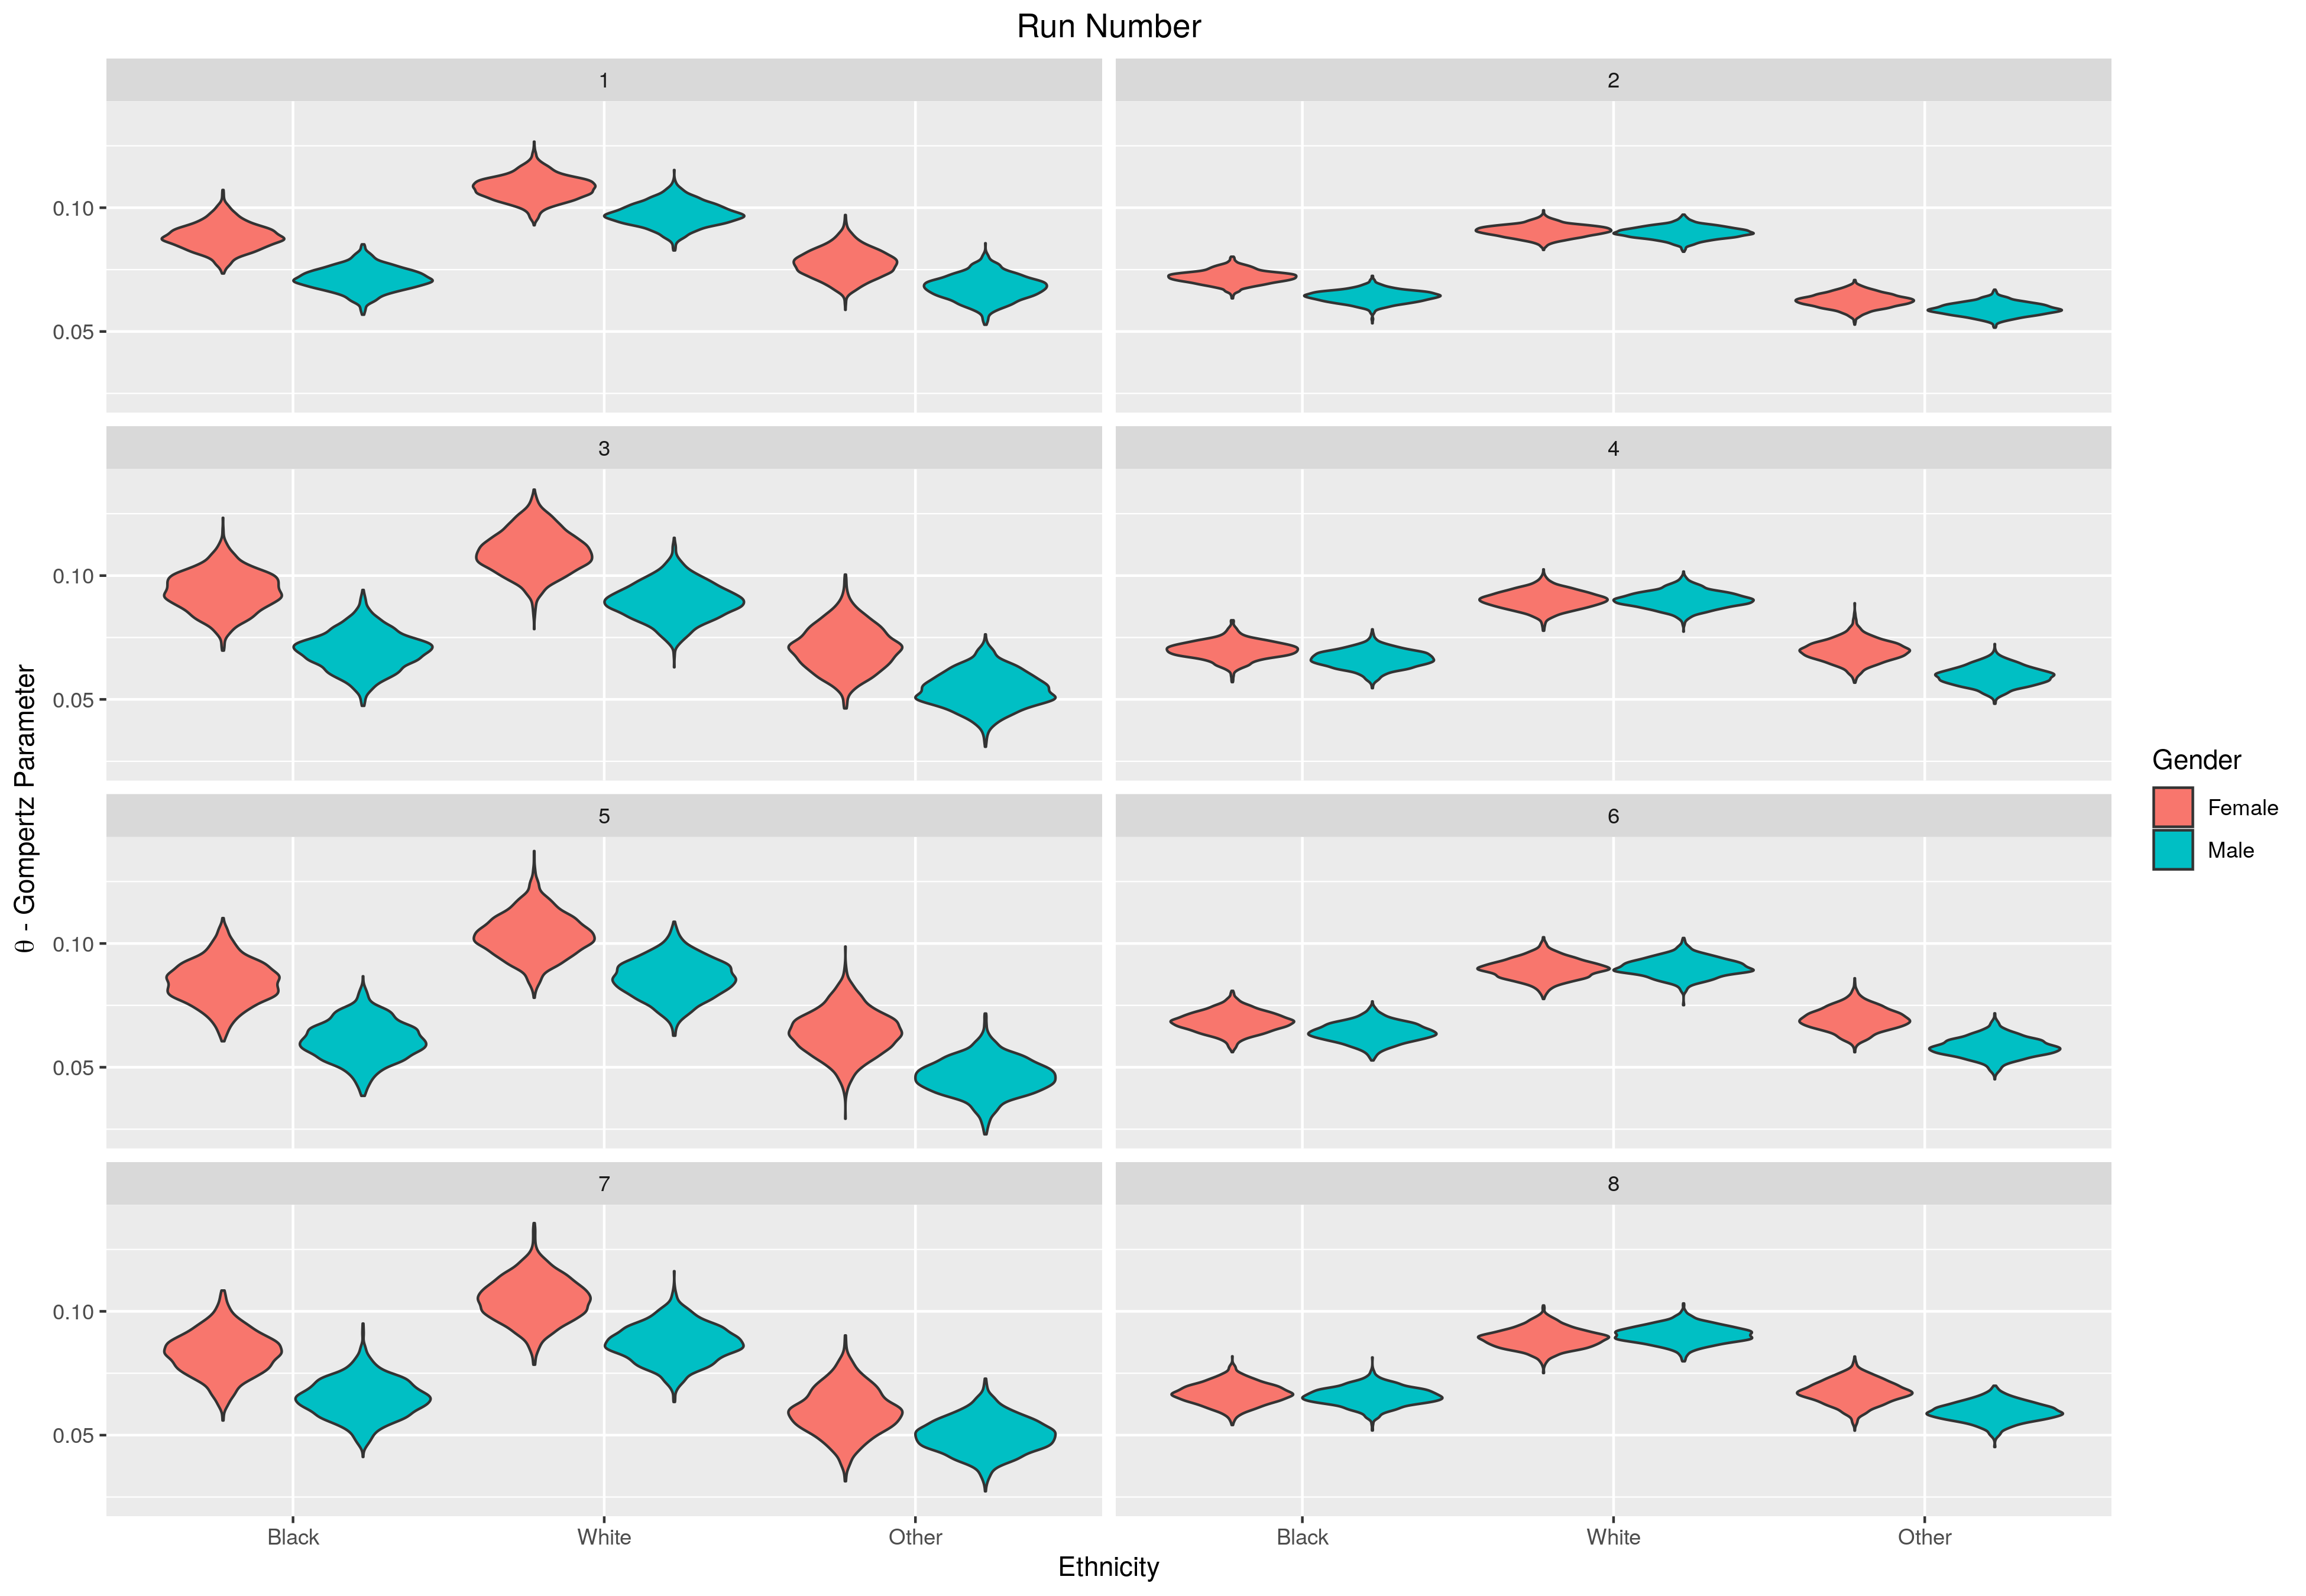
\includegraphics{../Plots/gompertz/theta_parameter.png} To measure the
performance of the model to predict the survival outcome of individuals
in the population, figure A.7 shows, ordered by individual age, the
cumulative hazard \(H(t)\) predicted against the cumulative number of
deaths in the populations, for each model explored in this research.
Each model is shown to predict survival outcomes reliably, across the
entire age range of the population.

\begin{figure}
\centering
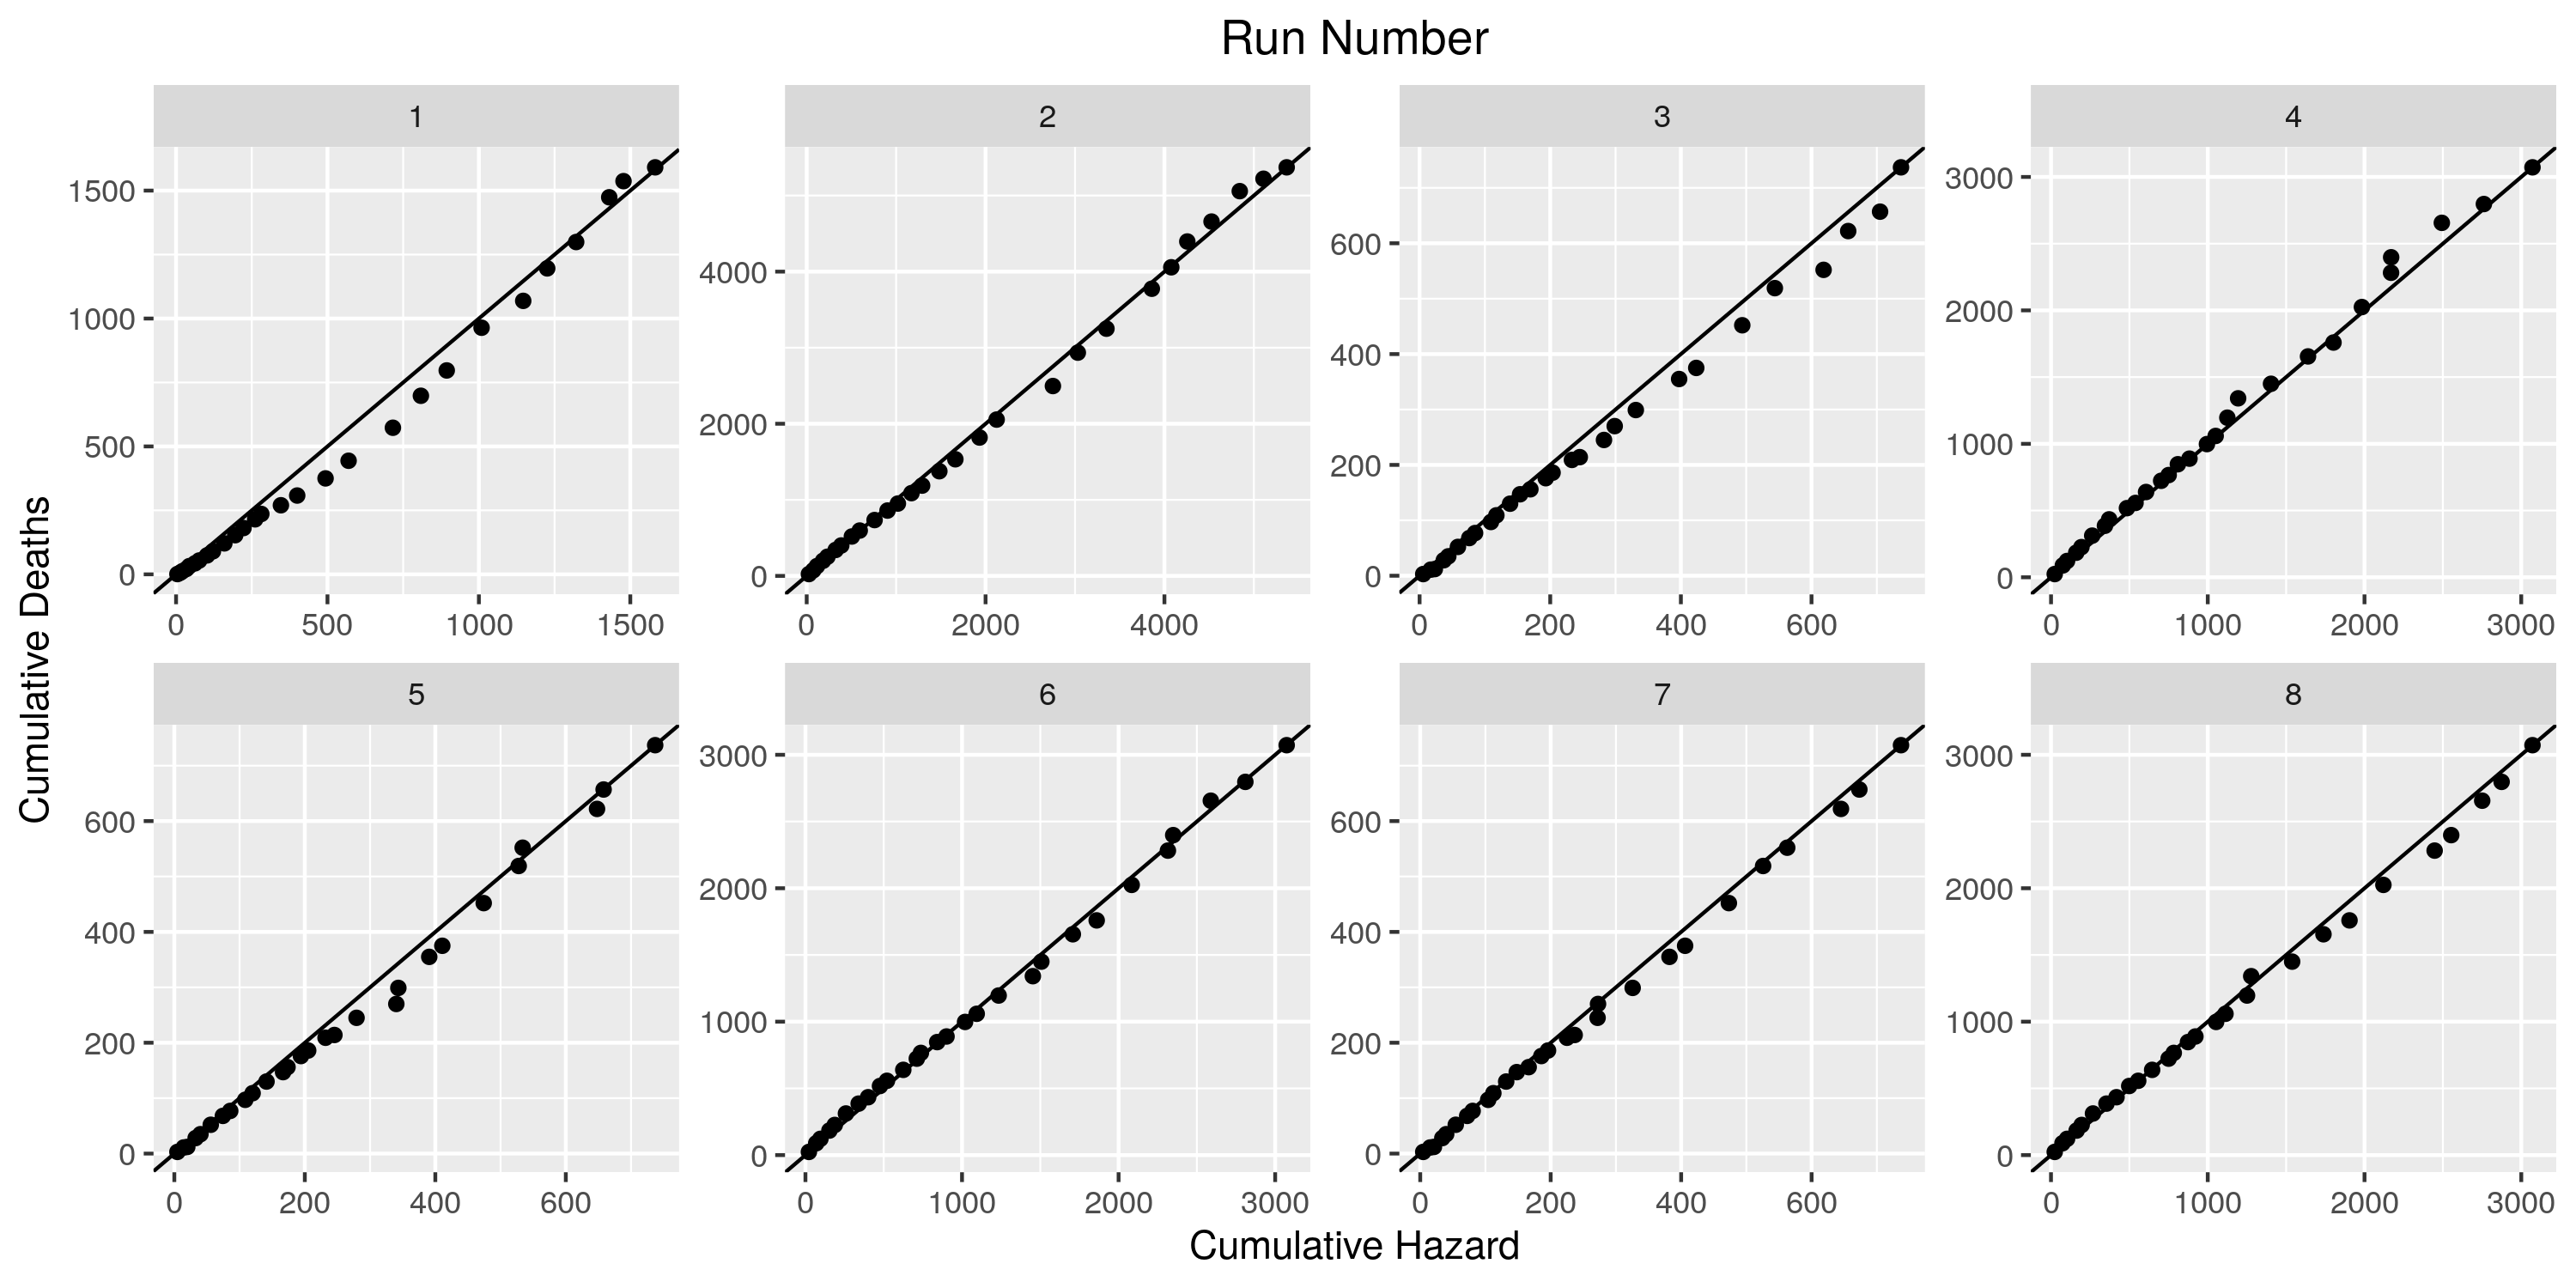
\includegraphics{../Plots/Survival/redlinpred_Cumulative_haz-death_age.png}
\caption{Figure A.7:}
\end{figure}

\end{document}
